\chapter{Vergleich der Cloud-Kosten}

Im folgenden Kapitel werden die monatlich anfallenden Cloud-Kosten \autocite{awsPricing} \autocite{gcpPricing} für die entwickelte Software am Standort Frankfurt verglichen. Die verwendeten Cloud-Dienste kommen aus der Architektur. Außerdem stellt das Kapitel ein Nutzungsszenario für eine Video-Plattform vor, um zu ermitteln, für welchen Fall welcher Dienst wirtschaftlicher ist. Zunächst folgt die Auflistung der Kosten in unterschiedliche Kategorien.

\section{Hosting-Kosten}

\begin{figure}%
    \centering
    \subfloat[\centering Gespeicherte Daten]{{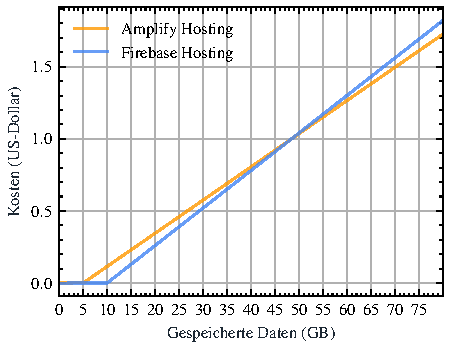
\includegraphics[width=6cm]{7_2_vergleich-cloud-kosten/hosting-stored-data.pdf} }}%
    \qquad
    \subfloat[\centering Übertragene Daten]{{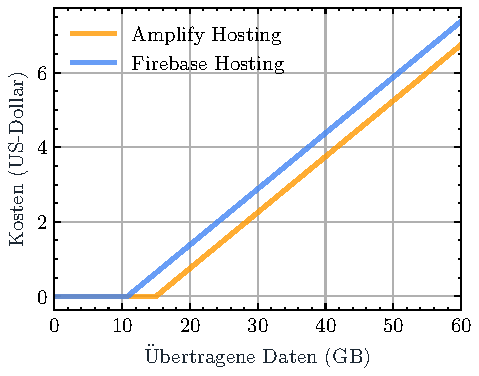
\includegraphics[width=6cm]{7_2_vergleich-cloud-kosten/hosting-transferred-data.pdf} }}%
    \caption{Kostenvergleich zwischen Amplify Hosting und Firebase Hosting}%
    \label{kostenvergleichHosting}%
\end{figure}

Beide Dienste benötigen den Hosting-Dienst, um das jeweilige Frontend zu speichern und zu übertragen. Dabei fallen Kosten für die Menge der gespeicherten Daten als auch für die Menge der übertragenen Daten an. \autoref{kostenvergleichHosting} stellt diesen Sachverhalt pro Kostenart dar.

\begin{description}
  \item[Gespeicherte Daten] Für das Amplify Hosting fallen \$ 0,023 pro GB an. Die ersten 5 GB sind kostenfrei. Für das Firebase Hosting fallen \$ 0,026 pro GB an. Die ersten 10 GB sind kostenfrei.
  \item[Übertragene Daten] Für beide Dienste fallen \$ 0,15 pro GB an. Lediglich das kostenlose Kontingent ist für das Amplify Hosting mit 15 GB gegenüber 10,8 GB für das Firebase Hosting etwas höher.
\end{description}

Für Projekte bis $\approx$ 48,33 GB sind die gespeicherten Daten in Firebase kostengünstiger. Für Projekte mit einem noch größeren Wert ist \ac{AWS} Amplify wirtschaftlicher. Bei Projekten mit bis zu 5 GB weist kein Tool einen Kostenvorteil aus, da beide noch kostenfrei sind. Die gespeicherten Daten hängen auch von der Anzahl der Builds ab. Demnach ist dieser Wert dann sinnvoll zu betrachten, wenn die Software hohe Entwicklungszyklen aufweist.

Die übertragenen Daten skalieren allerdings schneller als die gespeicherten Daten, da diese an die Anzahl der Nutzer gekoppelt sind, welche pro Aufruf ein Mal das Frontend herunterladen. Dabei ist kein wesentlicher Unterschied zwischen den beiden Diensten erkennbar, da das kostenlose Kontingent lediglich um 4,2 GB höher ist, was nur einen einmaligen Preisvorteil von maximal \$ 0,63 bringt.

Ein Vergleich der Build-Zeit findet an dieser Stelle nicht statt. \ac{AWS} Amplify selbst rechnet Build-Zeit mit \$ 0,01 pro Minute ab. Firebase Hosting bietet selbst keinen Build-Dienst als Gesamt-Deployment an. Daher muss dafür ein externer Dienst genutzt werden. Lediglich rechnet Google Cloud Functions die Dauer für das Deployment von einzelnen Funktionen ab.

Zusammenfassend lässt sich im Bereich Hosting kaum ein Kostenunterschied feststellen. Dies liegt daran, dass der  Proportionalitätsfaktor der übertragenen Daten bei beiden Diensten gleich ist.

\section{Computing-Kosten}

\begin{figure}
  \centering
  \subfloat[][\centering Ausführungszeit]{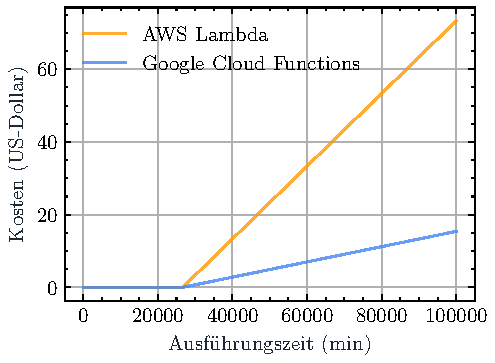
\includegraphics[width=.4\textwidth]{7_2_vergleich-cloud-kosten/functions-compute.pdf}}\quad
  \subfloat[][\centering Funktionsaufrufe]{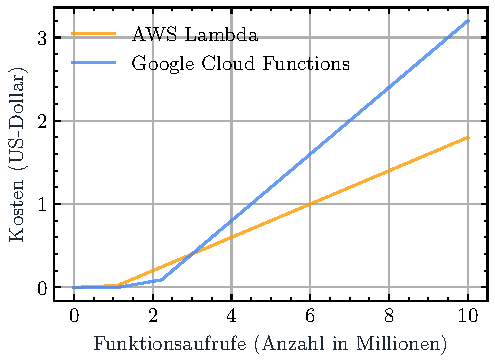
\includegraphics[width=.4\textwidth]{7_2_vergleich-cloud-kosten/functions-invocation.pdf}}\\
  \subfloat[][\centering Ausgehender Netzwerktransfer]{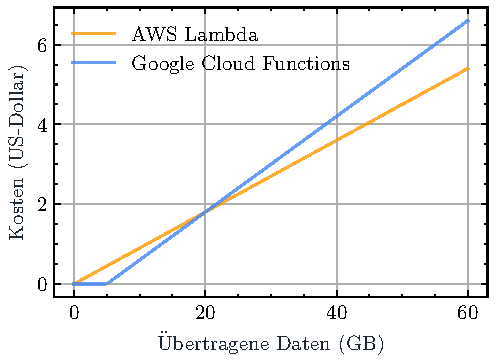
\includegraphics[width=.4\textwidth]{7_2_vergleich-cloud-kosten/functions-transfer.pdf}}\quad
  \caption{Kostenvergleich zwischen AWS Lambda und Google Cloud Functions}
  \label{kostenvergleichFunctions}
\end{figure}

Beide Dienste nutzen Funktionen, um die Logik der Software abzubilden. Die Kosten unterteilen sich dabei in Ausführungs-, Aufruf- und ausgehende Netzwerkkosten. \autoref{kostenvergleichFunctions} stellt diesen Sachverhalt pro Kostenart dar. Die Angaben basieren auf 256 MB Arbeitsspeicher und der dazu gehörigen CPU mit einem x86-Prozessor. Außerdem werden für die Google Cloud die Tier-2 Preise genutzt, da diese für den Datencenter in Frankfurt ausschlaggebend sind.

\begin{description}
  \item[Ausführungszeit] Für AWS Lambda fallen \$ 0,0000166667 pro GB-Sekunde an. Für Google Cloud Functions fallen \$ 0,0000175 pro GB-Sekunde an. Bei beiden Diensten sind die ersten 400000 GB-Sekunden kostenfrei. Im Preis von Google Cloud Functions sind die CPU-Preise mit einkalkuliert, da diese separat berechnet werden.
  \item[Funktionsaufrufe] Für AWS Lambda fallen \$ 0,20 pro Millionen Aufrufen an. Die ersten 1 Millionen Aufrufe sind kostenfrei. Für Google Cloud Functions fallen \$ 0,40 pro Millionen Aufrufen an. Die ersten 2 Millionen Aufrufe sind kostenfrei.
  \item[Ausgehender Netzwerktransfer] Da in der entwickelten Software die Lambda-Funktionen von AppSync aufgerufen werden, gelten für den Netzwerktransfer die Preise dieses Services. Diese belaufen sich auf \$ 0,09 pro GB. Bei Google Cloud Functions sind es \$ 0,12 pro GB. Außerdem gibt es noch ein kostenloses Kontingent von 5 GB.
\end{description}

Die Ausführung von Funktionen mit \ac{AWS} Lambda und Google Cloud Functions ist ungefähr gleich. Lediglich kosten die Google Cloud Functions 5 Prozent mehr. Allerdings ist der direkte Vergleich irreführend, da die zu Grunde liegende Abrechnungsmethode beachtet werden muss. Während Lambda die Ausführungszeiten auf 1 ms rundet, wird bei Google Cloud Functions auf die nächsten 100 ms gerundet. Das bedeutet, dass eine Anfrage mit 10 ms auf 100 ms gerundet wird. Dabei würde dann das 10-fache der Nutzung bezahlt werden.

Auch bei den Funktionsaufrufen ist \ac{AWS} Lambda nach 3 Millionen Aufrufen nur halb so teuer wie Google Cloud Functions. Ein ähnliches Bild mit einem etwas geringeren Faktor ergibt sich bei dem Vergleich der Übertragungskosten.

Abgesehen vom kostenlosen Kontingent von Google Cloud Functions ist zusammenfassend \ac{AWS} Lambda wirtschaftlicher, da die Preise günstiger sind und auf Grund der besseren Rundung nur das bezahlt wird, was auch genutzt wird.

\section{Storage-Kosten}

\begin{figure}
  \centering
  \subfloat[][\centering Gespeicherte Daten]{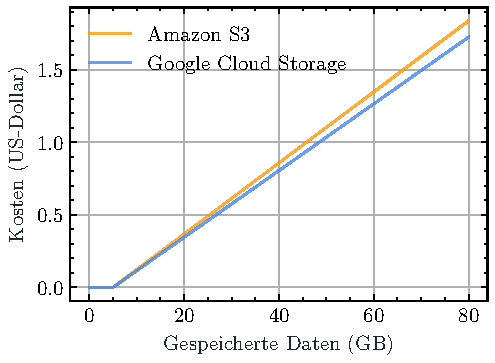
\includegraphics[width=.4\textwidth]{7_2_vergleich-cloud-kosten/storage-amount.pdf}}\quad
  \subfloat[][\centering Get-Anfragen]{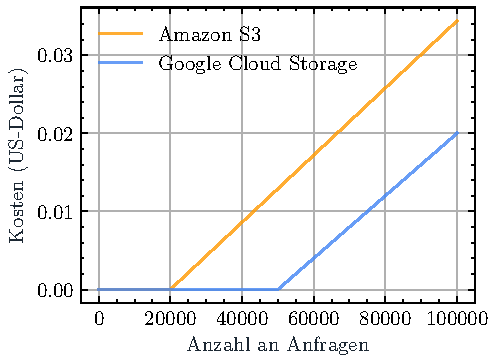
\includegraphics[width=.4\textwidth]{7_2_vergleich-cloud-kosten/storage-get.pdf}}\\
  \subfloat[][\centering Put/Post/List-Anfragen]{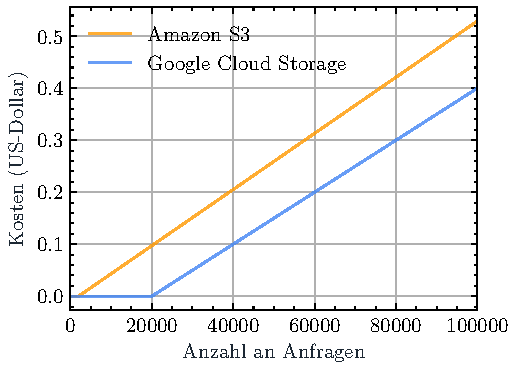
\includegraphics[width=.4\textwidth]{7_2_vergleich-cloud-kosten/storage-put.pdf}}\quad
  \subfloat[][\centering Ausgehender Netzwerktransfer]{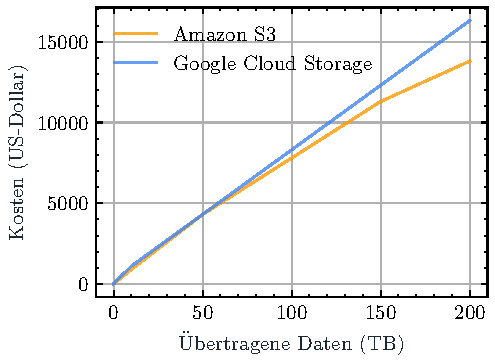
\includegraphics[width=.4\textwidth]{7_2_vergleich-cloud-kosten/storage-network.pdf}}
  \caption{Kostenvergleich zwischen Amazon S3 und Google Cloud Storage}
  \label{kostenvergleichStorage}
\end{figure}

Die Dienste nutzen den Storage für die Ablage der Videos. Die Kosten unterteilen sich in gespeicherte Daten, verschiedene Anfragearten sowie in Netzwerktransfer. Dabei ist der eingehende Netzwerktransfer bei beiden Anbietern kostenfrei, der ausgehende Transfer wird berechnet. In beiden Fällen werden zwei Anfragearten unterschieden: Get- und Select-Anfragen sowie Put, Post, Copy und List-Anfragen.

\begin{description}
  \item[Gespeicherte Daten] Für Amazon S3 fallen \$ 0,0245000000 pro GB an. Die ersten 5 GB sind kostenfrei. Für Google Cloud Storage fallen \$ 0,023 pro GB an. Dabei sind auch die ersten 5 GB kostenfrei.
  \item[Get-Anfragen] Anfragen dieser Kategorie kosten bei \ac{AWS} S3 \$ 0,00000043. Die ersten 20000 Anfragen sind kostenfrei. Für den Google Cloud Storage sind es \$ 0,0000004 pro Anfrage mit 50000 kostenfreien Anfragen.
  \item[Put-Anfragen] Diese Anfragen sind etwas teurer als Get-Anfragen. Bei \ac{AWS} S3 sind es \$ 0,0000054 mit 2000 kostenfreien Anfragen. Beim Google Cloud Storage sind es \$ 0,000005 mit 20000 kostenfreien Anfragen.
  \item[Ausgehender Netzwerktransfer] Bei \ac{AWS} S3 fallen für die ersten 10 TB \$ 0,09 pro GB an. Ab dann wird es stufenweise günstiger bis hin zu \$ 0,05 pro GB ab 150 TB. Beim Google Cloud Storage fallen \$ 0,12 pro GB an. Bis 10 TB sinkt der Preis auf \$ 0,11 bis hin zu \$ 0,08 ab 10 TB. Die ersten 30 GB sind dabei kostenfrei.
\end{description}

In den ersten drei Kategorien ist der Google Cloud Storage kostengünstiger. Die Netzwerkkosten sind bei \ac{AWS} abgesehen vom kostenlosen Kontingent von Google immer günstiger. Zusammenfassend ist damit die Google Cloud in der Kategorie Storage in den meisten Fällen kostengünstiger. Allerdings könnte sich für eine Video-Plattform, welche über 50 TB an Daten ausgibt, die mehr als 50 Prozent günstigeren ausgehenden Netzwerktransfer-Kosten positiv auswirken.

\section{Datenbank-Kosten}

\begin{table}[h]
  \caption{Kostenvergleich zwischen DynamoDB und Firestore}
  \label{KostenDatenbank}
  \renewcommand{\arraystretch}{1.2}
  \centering
  \sffamily
  \begin{footnotesize}
    \begin{tabularx}{0.9\textwidth}{l l l}
      \toprule
      \textbf{Kostenart} & \textbf{DynamoDB} & \textbf{Firestore}\\
      \midrule
      \emph{Gespeicherte Daten / GB (kostenfrei)} & \$ 0,306 (25 GB) & \$ 0,117 (1 GB) \\
      \emph{Lesezugriffe / 100k (kostenfrei)} & \$ 0,305  & \$ 0,39 (50k) \\
      \emph{Schreibzugriffe / 100k (kostenfrei)} & \$ 1,525  & \$ 1,17 (20k) \\
      \emph{Löschzugriffe / 100k (kostenfrei)} &  s. Schreiben & \$ 0,13 (20k) \\
      \emph{Netzwerktransfer / GB (kostenfrei)} & \$ 0,09 - AppSync & \$ 0,12 - \$ 0,08 (10 GB) \\
      \emph{Backup / GB} & \$ 0,1224 & s. Lesezugriff \\
      \bottomrule
    \end{tabularx}
  \end{footnotesize}
  \rmfamily
\end{table}

Die Kosten der Datenbank sind abhängig von der Nutzung der Dienste. Unterschieden wird hier wie in \autoref{KostenDatenbank} dargestellt zwischen in der Datenbank gespeicherte Daten, Lesezugriffe, Schreib- und Löschzugriffe sowie den ausgehenden Netzwerktransfer. Zur besseren Vergleichbarkeit werden für DynamoDB die Preise für den Schreibzugriff \texit{Standard} und den Lesezugriff \textit{strongly consistent}. Dies entspricht auch den Eigenschaften von Firebase.

Dennoch ist ein direkter Vergleich der beiden Datenbanken schwierig, da die Kosten für die Lese- und Schreibzugriffe bei DynamoDB abhängig von der Größe der Anfrage sind. Bei DynamoDB werden beim Schreiben mit bis zu 1 KB eine Einheit verrechnet. Überschreitet die Anfrage diesen Wert, werden entsprechend mehr Einheiten bezahlt. Beim Lesen ist das ähnlich. Lediglich wird dabei mit 4 KB pro Einheit gerechnet.

Vergleichbar sind allerdings die gespeicherten Daten. Diese sind für DynamoDB um ein Vielfaches teurer als für Firestore. Der Netzwerktransfer ist bis ungefähr 10 TB bei DynamoDB günstiger. Ab dann kostet Firestore nur \$ 0,08 pro GB. Allerdings wäre DynamoDB ohne AppSync dauerhaft günstiger, allerdings ist es aus Architektur-Sicht ein Vorteil, dass es eine GraphQL-Schnittstelle gibt, da diese noch weitere Logik bieten kann. Die Backup-Kosten sind bei DynamoDB günstiger, da dort per GB abgerechnet wird, während bei Firestore pro Datensatz ein fixer Betrag berechnet wird.

Alles in allem lässt sich beim Thema Datenbank an dieser Stelle nicht eindeutig sagen, welcher Dienst wirtschaftlicher ist. Das liegt daran, dass es auf den Use-Case und die genauen Werte ankommt und die Vergleichbarkeit auf Grund von unterschiedlichen Preismodellen nicht vollständig gegeben ist.

\section{Videokonvertierungskosten}

\begin{figure}
  \centering
  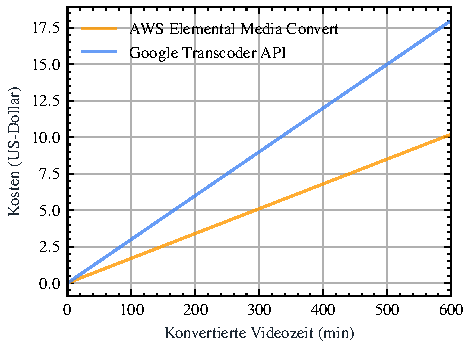
\includegraphics[width=0.75\columnwidth]{7_2_vergleich-cloud-kosten/transcoding.pdf}
  \caption{Kostenvergleich zwischen AWS Elemental Media Convert und Google Transcoder API}
  \label{KostenVideoTranscoding}
\end{figure}

Dieser Dienst wird genutzt, um das Wasserzeichen auf den hochgeladenen Videos zu platzieren. Die Werte beziehen sich auf die Konvertierung von Videos in HD-Qualität. Für \ac{AWS} Elemental Media Convert fallen \$ 0,017 pro Minute an. Für die Google Transcoder API fallen \$ 0,030 pro Minute an. \autoref{KostenVideoTranscoding} stellt diesen Zusammenhang dar. In diesem Bereich schneidet \ac{AWS} für jede Dauer besser ab.

\section{Sonstige Kosten}

Zu beachten ist zuletzt, dass einige Dienste für \ac{AWS} Amplify benötigt werden, die in Firebase nicht vorhanden sind oder in beiden Diensten nicht abgerechnet werden.
\begin{description}
\item[User Management] Da die erweiterten Sicherheitsfunktionalitäten von \ac{AWS} Cognito nicht genutzt werden, ist dieser kostenfrei. Auch seitens Firebase gibt es für das User-Management keine extra Kosten für die Standardfunktionalität.
\item[Benachrichtigung von Diensten] Amazon EventBridge wird verwendet, um \ac{AWS} Lambda darüber zu benachrichtigen, dass ein Video erfolgreich konvertiert wurde. Der Dienst kostet pro 1 Millionen Custom Events \$ 1,00. In Firebase ist dafür kein zusätzlicher Dienst nötig.
\item[GraphQL] Aufgrund von Unterschieden in der Architektur nutzt \ac{AWS} Amplify mit AWS AppSync einen GraphQL-Server, während Firebase ohne einen solchen auskommt, da Funktionen direkt aus dem Frontend aufgerufen werden können. Bei \ac{AWS} entstehen dadurch Nutzungskosten von \$ 4,00 für 1 Millionen Queries oder Mutations. Die ersten 250.000 Aufrufe sind dabei kostenfrei. Außerdem entstehen Datentransferkosten. Diese sind allerdings schon durch die Netzwerkkosten aus \ac{AWS} Lambda abgedeckt.
\end{description}

\section{Nutzungsszenario}

Der letzte Abschnitt stellt ein Nutzungsszenario für die entwickelte Video-Plattform dar. \autoref{ParameterNutzungsszenario} definiert die Eingangsparameter für die Berechnung. Dies entspricht einer Video-Plattform, welche täglich aktualisiert wird,  500.000 Nutzer hat und jeder Nutzer durchschnittlich 30 Videos im Monat schaut. Das Szenario setzt damit vor allem einen Fokus auf Plattformen mit vielen Bild- und Videoaufrufen.

\begin{table}[h]
  \caption{Eingangsparameter des Nutzungsszenarios}
  \label{ParameterNutzungsszenario}
  \renewcommand{\arraystretch}{1.2}
  \centering
  \sffamily
  \begin{footnotesize}
    \begin{tabularx}{0.9\textwidth}{l l l}
      \toprule
      \textbf{Parameter} & \textbf{Wert}\\
      \midrule
      \emph{Größe des Frontend-Builds} & 5 MB \\
      \emph{Nutzer pro Monat} & 500.000 \\
      \emph{Deployments pro Monat } & 30 \\
      \emph{Anzahl an Videoauflistungen pro Monat} & 5.000.000 \\
      \emph{Anzahl an aufgerufenen Videos pro Monat} & 15.000.000 \\
      \emph{Anzahl an hochgeladenen Videos pro Monat} & 1.800 \\
      \emph{Anzahl an aktualisierten Videos pro Monat} & 1.000 \\
      \emph{Anzahl an gelöschten Videos pro Monat} & 10 \\
      \emph{Durchschnittliche Funktionsdauer} & 0,25 sec \\
      \emph{Durchschnittlicher Verbrauch pro Funktion} & 256 MB \\
      \emph{Durchschnittliche Netzwerknutzung pro Funktion} & 2 KB \\
      \emph{Gespeicherte Videos} & 100.000 \\
      \emph{Durchschnittliche Video-Größe in MB} & 50 MB \\
      \emph{Durchschnittliche Video-Länge} & 1 min \\
      \emph{Durchschnittliche Größe in Datenbank} & 1 KB \\
      \bottomrule
    \end{tabularx}
  \end{footnotesize}
  \rmfamily
\end{table}

\autoref{BerechnungNutzungsszenario} zeigt die dazugehörigen Kosten. Die Berechnung erfolgt mit Kalkulation der Netto-Preise in US-Dollar inklusive kostenloser Kontingente. Für die Berechnung sind folgende Aspekte zu beachten:

\begin{itemize}
  \item Für die Computing-Zeit wurden bei \ac{AWS} Amplify die Anzahl der Videoauflistungen und der hochgeladenen sowie aufgerufenen Videos angenommen. Die Anzahl der aktualisierten und gelöschten Videos läuft nicht über eine Funktion sondern geht direkt auf die Datenbank mittels eines VTL-Resolvers von \ac{AWS} AppSync aus. Bei Firestore ist dies nicht der Fall. Hier fließen alle Metriken mit in die Computing-Zeit ein.
\end{itemize}

zwischenschritte

\begin{table}[h]
  \caption{Berechnung des Nutzungsszenarios}
  \label{BerechnungNutzungsszenario}
  \renewcommand{\arraystretch}{1.2}
  \centering
  \sffamily
  \begin{footnotesize}
    \begin{tabularx}{0.9\textwidth}{l r r}
      \toprule
      \textbf{Kostenart} & \textbf{AWS Amplify} & \textbf{Firebase}\\
      \midrule
      \emph{Hosting - Gespeicherte Daten} & \$ 0,00  & \$ 0,00 \\
      \emph{Hosting - Übertragene Daten} & \$ 372,75 & \$ 373,38 \\
      \emph{Computing - Funktionsdauer} & \$ 13,96 & \$ 14,66 \\
      \emph{Computing - Funktionsaufrufe} & \$ 2,80 & \$ 2,60 \\
      \emph{Computing - Ausgehende Netzwerktransfer} & \$ 2,70 & \$ 0,00 \\
      \emph{Storage - Gespeicherte Daten} & \$ 122,50 & \$ 115,00 \\
      \emph{Storage - Get-Anfragen} & \$ 0,00 & \$ 0,00 \\
      \emph{Storage - Put-Anfragen} & \$ 6,44 & \$ 5,98 \\
      \emph{Storage - Ausgehender Netzwerktransfer} & \$ 42.291,20 & \$ 61.757,36 \\
      \emph{Datenbank - Gespeicherte Daten} & \$ 0,00 & \$ 0,00 \\
      \emph{Datenbank - Lesezugriffe} & \$ 45,75 & \$ 58,31 \\
      \emph{Datenbank - Schreibzugriffe} & \$ 0,04 & \$ 0,00 \\
      \emph{Datenbank - Löschzugriffe} & \$ 0,00 & \$ 0,00 \\
      \emph{Datenbank - Ausgehender Netzwerktransfer} & \$ 1,35 & \$ 0,60 \\
      \emph{Datenbank - Backup} & \$ 0,01 & \$ 0,00 \\
      \emph{Video-Transkodierung} & \$ 30,60 & \$ 54,00 \\
      \emph{Event-Übertragungen} & \$ 1,00 & n. v. \\
      \emph{GraphQL-Service} & \$ 59,02 & n. v. \\
      \emph{} &  &  \\
      \textbf{Summe} & \$ 42.950,12 & \$ 62.381,89 \\
      \bottomrule
    \end{tabularx}
  \end{footnotesize}
  \rmfamily
\end{table}

\section{Zusammenfassung}

zusammenfassung aller dienste und wo welcher dienst günstiger ist